\documentclass[%
 reprint,
%superscriptaddress,
%groupedaddress,
%unsortedaddress,
%runinaddress,
%frontmatterverbose, 
%preprint,
%preprintnumbers,
nofootinbib,
%nobibnotes,
%bibnotes,
 amsmath,amssymb,
 aps,
 prd,
%pra,
%prb,
%rmp,
%prstab,
%prstper,
floatfix,
]{revtex4-2}

\usepackage{graphicx}
\usepackage{bm}
\usepackage{hyperref}
\usepackage[utf8]{inputenc}
\usepackage[cal=boondoxo]{mathalfa}
\usepackage[ruled, linesnumbered]{algorithm2e}
\usepackage[english]{babel}

%tables 
\usepackage{booktabs}
\renewcommand{\arraystretch}{1.2} 


%commutative diagrams
\usepackage{tikz,tikz-3dplot}
\tdplotsetmaincoords{90}{45}
\tdplotsetrotatedcoords{-90}{180}{-90}

%drawing cones
\tikzset{surface1/.style={draw=black, fill=gray, fill opacity=.30}}
\newcommand{\coneback}[4][]{
  \draw[canvas is xy plane at z=#2, #1] (45-#4:#3) arc (45-#4:225+#4:#3) -- (O) --cycle;
  }
\newcommand{\conefront}[4][]{
  \draw[canvas is xy plane at z=#2, #1] (45-#4:#3) arc (45-#4:-135+#4:#3) -- (O) --cycle;
  }

%theorem environment
\usepackage{amsthm}
\newtheorem{theorem}{Theorem}
\newtheorem{definition}{Definition}

%citation nasa ads macros
\def\apjl{\textit{ApJ}}                % Astrophysical Journal, Letters
\def\apj{\textit{ApJ}}                % Astrophysical Journal, 
\def\aj{\textit{AJ}}                % Astronomical Journal, 
\def\aap{\textit{A\&A}}              % Astronomy & Astrophysics
\def\prd{\textit{Phys.~Rev.~D}}        % Physical Review D
\def\prl{\textit{Phys.~Rev.~Lett.}}    % Physical Review Letters
\def\jcap{\textit{J. Cosmology Astropart. Phys.}}
                % Journal of Cosmology and Astroparticle Physics
                


\begin{document}

\preprint{APS/123-QED}

\title{Perturbative Approach to Covariant Constructive Gravity}

\author{Tobias Reinhart}
\email{tobi.reinhart@fau.de}
\author{Nils Alex}
\affiliation{Department Physik, Friedrich-Alexander Universit{\"a}t Erlangen-N{\"u}rnberg,\\
91058 Erlangen, Germany}


\begin{abstract}
We propose a general framework for the construction of alternative theories of gravity, perturbatively as well as in the exact setting. The construction is guided by no more than two fundamental principles that we impose on the to-be-constructed gravitational dynamics: their invariance under spacetime diffeomorphisms and the compatibility of their causal structure with given given matter dynamics, provided that spacetime is additionally endowed with a matter field. The developed framework then allows to compute the most general, alternative theory of gravity that is consistent with the two fundamental requirements. We explicitly test this in the perturbative setting, by deriving the most general third order expansion of a metric theory of gravity that is compatible with a Klein-Gordon scalar field. Thereby we recover the corresponding third order expansion of General Relativity. Moreover we construct the most general third order perturbative theory of gravity that is capable of supporting a linear theory of electrodynamics.
\end{abstract}

\keywords{alternative theories of gravity, diffeomorphism invariance, classical field theory, causality}
\maketitle

\section{Introduction}
Measurements of the expansion of the universe (cf. \cite{1999ApJ...517..565P} and \cite{1998AJ....116.1009R}) as well as observations of galaxy rotation curves (\cite{1970ApJ...160..811F}, \cite{1970ApJ...159..379R} and \cite{1980ApJ...238..471R}) are only consistent with General Relativity if one subjects Einstein's theory to modifications, i.e., supplements it with additional field content. Although these modifications --- commonly known as dark energy and dark matter --- are widely accepted, it seems unsavory that render an existing theory consistent with otherwise contradicting experiments by ad hoc modifying its content. Reasonable doubt concerning this procedure got further amplified when the Planck mission revealed that these ad hoc modifications are in no way marginal, as when basing predictions on the cosmological standard model, dark matter compromises an astonishing $ 25.8\pm0.4\%$ of the observable universe's energy content, whereas dark energy even accounts for $ 69 \pm 1 \%$ of it (cf. \cite{Planck13_1}, \cite{Planck13_2}, \cite{Planck15} and \cite{Planck18}). Thus these two ad hoc modifications in the end describe roughly $95\%$ of the theories content. 

Although since this discovery, numerous proposed alternatives to GR (\cite{Scalar1}, \cite{Scalar2}, \cite{ST1}, \cite{ST2}, \cite{ST3},\cite{SVT1}, \cite{SVT2}, \cite{fR1}, \cite{fR2}, \cite{BIM1}, \cite{BIM2}) tried to resolve this inconsistency, recently there has been no real breakthrough in this area of research. The problem of constructing alternative theories of gravity is foremost plagued by the sheer infinite number of possibilities for describing gravity.  To that end the problem of constructing alternative theories of gravity should best be tackled with a more structured plan at hand.

One such plan is precisely what we wish to propose in this paper. more precisely, we are going to impose two fundamental requirements on any theory of gravity: 

\begin{samepage}
\begin{itemize}
    \item[\textbf{\textit{(A1)}}] \textbf{\textit{The dynamical laws that govern gravity are invariant under spacetime diffeomorphisms.}}
    \item[\textbf{\textit{(A2)}}] \textbf{\textit{Provided that spacetime is additionally inhabited by matter fields, their dynamics is causally compatible with the gravitational dynamics.}}
\end{itemize}
\end{samepage}

Any further results that we are going to present are then simply implications of these requirements. In particular, we are going to outline how these requirements can be employed to construct, for the general case of the gravitational field being described by any tensor field at wish, the most comprehensive dynamical theory of gravity that is consistent with the two fundamental requirements. 

We structure the paper as follows: 
In the beginning of chapter \ref{chapter1} we develop the necessary tools to obtain a rigorous formulation of gravity as a second order Lagrangian field theory phrased in terms of the jet bundle framework. We then proceed by  two fundamental requirements into precise mathematical language, condition (A1) is shown to require the gravitational Lagrangian to obey a specific linear first order system of partial differential equations, whereas condition (A2) can be incorporated by imposing additional conditions on the principal polynomial of the gravitational EOM. 

In chapter \ref{chapter2} we deduce perturbative equivalents to the two fundamental requirements that we phrased in chapter \ref{chapter1}. On top of that we concern our selves with the computation of power series solution the PDE that we derived from (A1) in chapter \ref{chapter1}. This allows us to extract viable information regarding the number of independent curvature invarinats a given tensorial spacetime geometry admits, recovering the known number of $14$ curvature invariants for the case of spacetime being endowed with a metric structure. 

Finally, the second chapter culminates with a concrete, algorithmic manual for the (perturbative) construction of gravity theories that we will put to test in the third and final chapter.


\section{The Axioms of Constructive Gravity}\label{chapter1}
\subsection{A1: Diffeomorphism Invariant Gravitational Dynamics }

We wish to describe the gravitational field as a tensor field\footnote{The following developments can readily be generalized to the case of describing the gravitational field as a section of any bundle that is associated to the frame bundle, i.e., any natural bundle (cf. \cite{kolar1993natural}).} over the $4$-dimensional spacetime manifold $M$. To that end let $F \subset T^m_nM$ be a vector subbundle of the $(m,n)$ tensor bundle over $M$, such that the gravitational field can be described as a section $G \in \Gamma(F)$ of this bundle, the \textit{\textbf{gravitational field bundle}}. 
We denote adapted coordinates\footnote{As $F$ is a vectorbundle we can and will always restrict to coordinates that are linear on the fibers (cf. \cite{saunders_1989}).} on $F$ by $(x^m,v_A)$, where we introduced the abstract index $A$ that consequently runs over the fiber dimension of $F$.

As $F$ defines a vector bundle we can define its vector bundle dual $F^{\ast}$ with fiber at $p\in M$ given by the vector space dual of $\pi_F^{-1}(p)$.
Moreover, we denote fiber coordinates dual to $v_A$ by $v^A$, i.e, these two sets of coordinate functions satisfy:
\begin{align}
    v^Av_B = \delta^A_B.
\end{align}

We might very well consider the case where $F$ represents a true subbundle of $T^m_nM$ and hence admits fibers of dimension $r < m+n$. For such situations it is convenient to introduce vector bundle morphisms that relate fiber coordinates $v_A$ on $F$ to fiber coordinates $v^{a_1 ... a_m}_{b_1 ... b_n}$ on $T^m_nM$.

\begin{definition}[intertwiner]\label{interDef}
Let $(F,\pi_F,M)$ be a vector bundle. We call a pair of vector bundle morphisms $(I, J)$:
\begin{align}
    \begin{aligned}
    I&: F \longrightarrow T^m_n M\\
    J&: T^m_n M \longrightarrow F 
    \end{aligned}
\end{align}
that cover $id_M$ and satisfy
$J \circ I = \mathrm{id}_F$ a pair of \textbf{\textit{intertwiners}} for the bundle $(F, \pi_F, M)$.
\end{definition}

These intertwiners relate fiber coordinates on $F$ to fiber coordinates on $T^m_nM$

\begin{align} \label{interRel1}
    \begin{aligned}
    & v^{a_1 ... a_m}_{b_1 ... b_n} & = & \ \ I^{A a_1 ... a_m}_{b_1 ... b_n} \cdot v_{A},\\  
    & v_A & = & \ \ J^{b_1 ... b_n}_{A a_1 ... a_m} \cdot v^{a_1 ... a_m}_{b_1 ... b_n},
    \end{aligned}
\end{align}

as well as fiber coordinates on $F^\ast$ to fiber coordinates on $T^n_mM$

\begin{align} \label{interRel2}
    \begin{aligned}
    & v^{b_1 ... b_n}_{a_1 ... a_m} & = & \ \ J^{b_1 ... b_n}_{A a_1 ... a_m} \cdot v^{A},\\  
    & v^A & = & \ \  I^{A a_1 ... a_m}_{b_1 ... b_n} \cdot v^{b_1 ... b_n}_{a_1 ... a_m}.
    \end{aligned}
\end{align}

The identity $J\circ I = \mathrm{id}_F$ reads in this coordinate representation
\begin{equation}
    \delta^A _ B \ \ = \ \ I^{A a_1 ... a_m}_{b_1 ... b_n} \cdot J^{b_1 ... b_n}_{B a_1 ... a_m}.  
\end{equation}

The dynamics of the gravitational field shall be encoded as equations of motion to a second-derivative-order \textit{\textbf{Lagrangian}} for the gravitational field. We deliberately restrict to second-derivative-order Lagrangians as any higher-derivative-order contribution necessarily also contributes to the equations of motion in higher than second derivative order. These contributions would then, however, yield to instabilities in the associated Hamiltonian formulation (cf. \cite{Ostrogradsky:1850fid}, \cite{2015arXiv150602210W}). 

Such a gravitational Lagrangian can be rigorously defined by utilizing the \textit{\textbf{jet bundle}} (cf.  \cite{saunders_1989}, \cite{seiler1994analysis}, \cite{seiler2009involution}, \cite{kolar1993natural},\cite{Gotay1992StressEnergyMomentumTA}, \cite{1998physics...1019G}). 
We denote adapted coordinates of the second order jet bundle $J^2F$ over $F$ by $(x^m, v_A, v_{Ap}, v_{AI})$. Here we introduced a new type of abstract indices that is used to label second order spacetime derivatives and thus, using that partial derivatives commute, runs from $0$ to $9$. 
The relation to the spacetime derivatives in standard notation is provided by an additional pair of intertwiners for the symmetric bundle $S_2M\subset T^0_2M$:
\begin{align}
    \begin{aligned}
        v_{AI} &= J_I^{ij} v_{Aij}\\
    v_{Aij} &= I^I_{ij} v_{AI}.
    \end{aligned}
\end{align}
We can now define a second-derivative-order gravitational Lagrangian as follows.
\begin{definition}[Lagrangian]
A second-order Lagrangian on $(F,\pi_F,M)$ is a bundle map that covers $id_M$:
\begin{align}
    \mathcal{L} : J^2F \longrightarrow \Lambda^4M.
\end{align}
\end{definition}
Thus the formulation of classical Lagrangian field theory yields the following situation, that can be seen in figure \ref{diagram1}:
\begin{figure}[hbt!]
\centering
\begin{tikzpicture}[scale=0.5]
\node (M) at (0,0) {$M$};
\node (F) at (0,2) {$F$};
\node (J1) at (0,4) {$J^1F$};
\node (J2) at (0,6) {$J^2F$};
\node (Vol) at (6,6) {$\Lambda^4M$};
\draw [-latex] (F) -- node[pos=0.35, right] {$\pi_F$} (M);
\draw [-latex] (J1) -- node[pos=0.35, right] {$\pi_{1,0}$}  (F);
\draw [-latex] (J2) -- node[pos=0.35, right] {$\pi_{2,1}$}  (J1);
\draw [-latex] (Vol.220) -- node[pos=0.4, left] {$\pi_{\Lambda^4M}$ \ }  (M.60);
\draw[-latex] (M) .. controls (-0.75,0.5) and (-0.75,1.5) .. node[pos=0.5, left] {$G$} (F);
\draw[-latex] (M) .. controls (-3,1) and (-3,5) .. node[pos=0.5, left] {$j^2(G)$} (J2);
\draw [-latex] (J2) -- node[pos=0.5, above] {$\mathcal{L}$}  (Vol);
\draw[-latex] (M.30) -- node[pos=0.5, right] { \ $\mathcal{L}\circ j^2(G)$} (Vol.250);
\end{tikzpicture}
\caption{Commutative Diagram: Lagrangian Field Theory on $J^2F$.} \label{diagram1}
\end{figure}
The gravitational field is described as a section of a bundle $F$ over the spacetime manifold $M$. As such it can be prolonged to any jet bundle $J^qF$, constructed over $F$, by applying the \textit{\textbf{jet prolongation}} map $j^q$. 
The Lagrangian $\mathcal{L}$ is a volume-form-valued bundle map on $J^2F$. Therefore we can prolong a given field $G \in \Gamma(F)$ to $J^2F$ and apply $\mathcal{L}$ on it to obtain a volume form on $M$, which then can be integrated.
This defines the usual \textit{\textbf{local action functional}} on the space of fields:
\begin{align}
\begin{aligned}
    \mathcal{S}_{\mathcal{L}} : \Gamma(F) &\longrightarrow \mathcal{R} \\
    G &\longmapsto \mathcal{S}_{\mathcal{L}}[G] := \int \mathcal{L}(j^2(G)).
\end{aligned}
\end{align}
Equations of motion (EOM) can be obtained by equating the \textit{\textbf{variational derivative}} of the Lagrangian with zero:
\begin{align}
  0 = E^A = \frac{\delta \mathcal{L}}{\delta v_A} = 
  \frac{\partial\mathcal{L}}{\partial v_A} - D_p ( \frac{\partial \mathcal{L}}{\partial v_{Ap}}) 
  + D_p D_q J^{pq}_I (\frac{\partial \mathcal{L}}{\partial v_{AI}}).
\end{align}
Here we further introduced the jet bundle \textit{\textbf{total derivative}}, sometimes also called formal derivative, $D_p$.
Given a function $f$ on $J^1F$, applying $D_p$ yields a function on the second order jet bundle:
\begin{align}
    D_p f := \frac{\partial f}{\partial x^p} + v_{Ap} \cdot  \frac{\partial f}{\partial v_A} + v_{AI} I^{I}_{pq} \cdot \frac{\partial f}{ \partial v_{Aq}}.
\end{align}
Note in particular that the EOM of a second-order Lagrangian are in general given by a function on $J^4F$, as we wish to restrict to theories that allow for a meaningful Hamiltonian formulation, we will restrict, however, to those cases where $\mathcal{L}$ is \textit{\textbf{degenerate}}, s.t. the EOM are also of second derivative order. 


One of the fundamental requirements that we wish to pose on the yet to be constructed gravitational dynamics is their \textit{\textbf{invariance under spacetime diffeomorphisms}}. 
This can be understood as a consequence of Einstein's requirement of general covariance (cf. \cite{Stachel1993-STATMO-5}, \cite{Pooley} and also \cite{Norton1993-NORGCA}).
To that end it is necessary that we lift the standard action of $\mathrm{Diff}(M)$ to $J^2F$.
As $F$ was required to be a subbundle of a tensor bundle over $M$, the action of $\mathrm{Diff}(M)$ lifts naturally by the usual pushforward-pullback construction to an action of $\mathrm{Diff}(M)$ on $F$ by vector bundle isomorphisms.
In the following we denote the image of $\phi \in \mathrm{Diff}(M)$ under this lift by $\phi_F$.
In order to further lift this action to the jet bundle we need to introduce some additional techniques from the theory of jet bundles.
\begin{definition}[prolongation of morphisms]
Let $(F_1,\pi_{F_1},M)$ and $(F_2,\pi_{F_2},N)$ be bundles, $\phi : M \rightarrow N$ a diffeomorphism, $f : F_1 \rightarrow F_2$ a bundle morphism covering $\phi$. The $k$th-order jet bundle lift of $(f,\phi)$ is the unique  map $j^k(f):J^kF_1 \rightarrow J^kF_2$ that lets the diagram in figure \ref{ProlongMorph} commute.
\begin{figure}[hbt!]
\centering
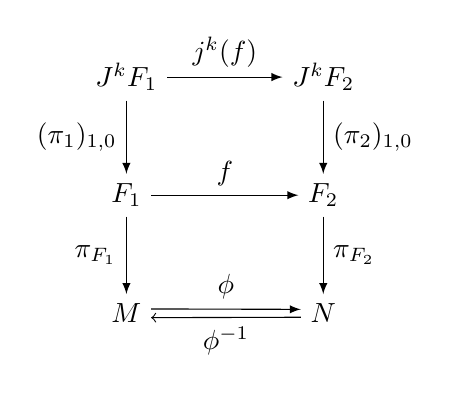
\begin{tikzpicture}[scale=0.5]
\node (M) at (0,0) {$M$};
\node (N) at (5,0) {$N$};
\node (F1) at (0,3) {$F_1$};
\node (F2) at (5,3) {$F_2$};
\node (JF1) at (0,6) {$J^kF_1$};
\node (JF2) at (5,6) {$J^kF_2$};
\draw [-latex] (M.10) -- node[pos=0.5, above] {$\phi$} (N.170);
\draw [<-] (M.350) -- node[pos=0.5, below] {$\phi^{-1}$} (N.190);
\draw [-latex] (F1) -- node[pos=0.5, above] {$f$} (F2);
\draw [-latex] (F1) -- node[pos=0.5, left] {$\pi_{F_1}$} (M);
\draw [-latex] (F2) -- node[pos=0.5, right] {$\pi_{F_2}$} (N);
\draw [-latex] (JF1) -- node[pos=0.5, left] {$(\pi_1)_{1,0}$} (F1);
\draw [-latex] (JF2) -- node[pos=0.5, right] {$(\pi_2)_{1,0}$} (F2);
\draw [-latex] (JF1) -- node[pos=0.5, above] {$j^k(f)$} (JF2);
\end{tikzpicture}
\caption{Commutative Diagram: Prolongation of Bundle Morphisms to First Jet Bundle.}\label{ProlongMorph}
\end{figure}
\end{definition}
Note that when acting on sections $G \in \Gamma(F_1)$, the jet bundle lift of bundle morphisms commutes with the jet prolongation map:
\begin{align}
j^k(f) \circ j^kG \circ \phi^{-1} = j^k \left (
f \circ G \circ \phi^{-1} \right ).
\end{align}

By using this notion of lifting bundle morhisms to the jet bundle we can finally formulate the first fundamental requirement of constructive gravity in rigorous fashion. 
\begin{definition}
A Lagrangian field theory described by a second-order Lagrangian $\mathcal{L} : J^2F \rightarrow \Lambda^4 M$ is called diffeomorphism invariant if $\mathcal{L}$ is equivariant w.r.t. the lifted action of $\mathrm{Diff}(M)$ on $J^2F$ and the pullback action on $\Lambda^4M$, i.e., if it holds for all $\phi \in \mathrm{Diff}(M)$ that 
\begin{align}\label{DiffeoReq}\tag{Axiom 1}
     \mathcal{L}\circ j^2(\phi_F) = \phi_{\ast} \circ \mathcal{L}.
\end{align}
\end{definition}

Infinitesimally, on the \textit{\textbf{Lie algebra level}}, diffeomorphisms are described by vector fields $\Gamma(TM)$ with lie bracket provided by their commutator. As usual we can obtain a Lie algebra ation from a given action of the corresponding Lie group (cf. \cite{boothby1989}, \cite{doi:10.1142/3867}).
This construction can in particular be used for the lifted action of $\mathrm{Diff}(M)$ on $F$ and on $J^2F$.
Doing so, we obtain a Lie algebra morphism:
\begin{align}\label{LieF}
\begin{aligned}
    \mathcal{f} : \Gamma(TM) &\longrightarrow \Gamma(TF)\\
    \xi &\longmapsto \xi_F \\
    \smallskip
    \xi_F = \xi^m \frac{\partial}{\partial x^m} + \xi^A \frac{\partial}{\partial v_A} &= \xi^m \frac{\partial}{\partial x^m} + C_{An}^{Bm} v_B \partial_m \xi ^n \frac{\partial}{\partial v_A}. 
\end{aligned}
\end{align}
Here we introduced the constant tensors $C^{Am}_{Bn}$ that describe the vertical coefficient of this lifted vector field.
Further, we get the following Lie algebra morphism that describes the corresponding vector field on $J^2F$:
\begin{align}
    \begin{aligned}
    j^2(\mathcal{f}) : \Gamma(TM) &\longrightarrow \Gamma(TJ^2F)\\
    \xi & \longmapsto \xi_{J^2F},
    \end{aligned}
\end{align}
where 
\begin{align}\label{LieJ2}
\begin{aligned}
    &\xi_{J^2F} = \xi^m \frac{\partial}{\partial x^m} + C_{An}^{Bm} v_B \partial_m \xi ^n \frac{\partial}{\partial v_A}
    + C_{An}^{Bm} \partial_m \xi^n v_{Bi} \frac{\partial}{\partial v_{Ai}}\\
    &\ \ - v_{An} \partial_m \xi ^n \frac{\partial}{\partial v_{Am}} + C_{An}^{Bm} v_B \partial_m \partial_p \xi^n \frac{\partial}{\partial v_{Ap}} \\
    & \ \ + C_{An}^{Bm} v_{BI} \partial_m \xi ^n \frac{\partial}{\partial v_{AI}}
    - 2 v_{BJ} I^J_{an}J^{am}_I \partial_m \xi^n \frac{\partial}{\partial v_{AI}}\\
    & \ \ + 2 C_{An}^{Bm} v_{Ba}J^{ap}_I \partial_m \partial_p \xi^n \frac{\partial}{\partial v_{AI}}
    - v_{An} J^{pm}_I \partial_m \partial_p \xi^n\frac{\partial}{\partial v_{AI}}\\
    & \ \ + C_{An}^{Bm} v_B J^{pq}_I \partial_m \partial_p \partial_q \xi^n \frac{\partial}{\partial v_{AI}}.
\end{aligned}
\end{align}
 
We can use the Lie algebra morphism (\ref{LieJ2}) to derive an infinitesimal version of the first fundamental requirement (\ref{DiffeoReq}).
\begin{theorem}
Let $\mathcal{L} = L \cdot \mathrm{d}^4x$ be the Lagrangian of a diffeormorphism invariant field theory on $J^2F$, i.e., $\mathcal{L}$ is assumed to satisfy condition (\ref{DiffeoReq}). Then the coordinate expression $L$ necessarily satisfies the following first-order, linear partial differential equation:  
\begin{align}\label{DiffeoEqn}
\begin{aligned}
    0 &= &&L_{:m} \\
    0 &= &&L^{:A} C_{An}^{Bm} v_B + L^{:Ap} \bigl[ C_{An}^{Bm} \delta_p^q - \delta_A^B \delta_m^n \bigr] v_{Bq}\\
    & &&+ L^{:AI} \bigl[ C_{An}^{Bm} \delta_I^J - 2 \delta_A^B J_I^{pm} I^J_{pn}  \bigr] v_{BJ} + L \delta^m_n \\
    0 &= &&L^{:A(p\vert}C_{An}^{B \vert m)} v_B + L^{: AI} \bigl[ C_{An}^{B(m\vert} 2 J_I^{\vert p) q} - \delta^B_A J_I ^{pm} \delta_n^q \bigr] v_{Bq} \\
    0 &= &&L^{:AI} C_{An}^{B(m\vert} v_B J_I^{\vert p q )}.
\end{aligned}
\end{align}
\end{theorem}
Here we introduced the notation $L_{:m} := \frac{\partial L}{\partial x^m}$, $L^{:A} := \frac{\partial L}{ \partial v_A}$, etc. .
\begin{proof}
Reexpressing condition (\ref{DiffeoReq}) infinitesimally, by utilizing the Lie algebra morphism (\ref{LieJ2}) for an arbitrary vector field $\xi \in \Gamma(TM)$, yields an equation with left-hand side given by applying $\xi_{J^2F}$ on $L$ and right-hand side given by the infinitesimal of the pullback action of $\phi$ on $\Lambda^4M$.
As $\xi \in \Gamma(TM)$ was assumed arbitrary we can chose the individual components s.t. we can isolate specific contributions to the equation. These then have to be satisfied independently. Several suitable choices for the vector field components then yield precisely the above PDE. 
\end{proof}

This system of $140$ first-order, linear partial differential equations for the Lagrangian follows necessarily from the requirement of diffeomorphism invariance. Therefore the notoriously difficult requirement of diffeomorphism invariant gravitational dynamics is translated into the much simpler condition that the gravitational Lagrangian be a solution to (\ref{DiffeoEqn}). Conversely, every solution to this PDE yields a valid candidate Lagrangian to describe the gravitational dynamics. 
The problem of constructing gravitational dynamics is thus rephrased as computing the general solution to (\ref{DiffeoEqn}). 
This is an enormous advantage. As solving partial differential equations is a frequently occurring problem in almost all areas of research, the underlying theory is extensively developed (cf. \cite{seiler2009involution}, \cite{hormander1994analysis}, \cite{hormander2009analysis}, \cite{hormander2015analysis}).
Moreover, many techniques how such equations might be solved have already been known for quite some time (see \cite{Hilbert}).

Furthermore, note that the only quantity appearing in (\ref{DiffeoEqn}) that explicitly depends on the specific nature of the gravitational field is the vertical coefficient of the Lie algebra action of diffeomorphisms on $M$. This allows for a unified treatment of the PDE, irrespective of the precise gravitational field at hand. 

Similar equations were already obtained in the context of variational calculus and gauge symmetries (cf. \cite{article}). 
Gotay et al. derived a similar system for the case of first-order Lagrangians (see \cite{Gotay1992StressEnergyMomentumTA} and \cite{1998physics...1019G}) and used it to define a universal, conserved energy-momentum-tensor as Noether current associated to $\mathrm{Diff}(M)$. 
Unfortunately, restricting to first-order Lagrangians for a description of gravity does not always suffice --- for instance it does not when formulating GR such that the usual metric tensor constitutes the only dynamical field.

There are many exciting implications of this diffeomorphism equivariance PDE that are , however, beyond the scope of this paper. We have already presented a framework of constructing perturbative gravitational dynamics that thrives on  consequences of (\ref{DiffeoEqn}) on the corresponding EOM (cf. \cite{TobiR}).
Utilizing Gotay et al.'s jet bundle based formulation of Hamiltonian dynamics (see \cite{2004math.ph..11032G}) one can further show --- at least for first-derivative-order theories --- that the Hamiltonian associated to any diffeomorphism invariant Lagrangian field theory is necessarily given by a linear combination of $4$ primary and $4$ secondary constraints and thus vanishes weakly ( cf. \cite{TobiMaster}).

Finally, it is worth noting that diffeomorphism invariance also constitutes the main guiding principle for three well-known approaches that achieved to recover Einstein's General Relativity as the unique, second-derivative-order, metric theory of gravity. 
First of all, Loverlock (see \cite{Lovelock1969}, \cite{doi:10.1063/1.1665613} and \cite{doi:10.1063/1.1666069}), by directly imposing the condition of diffeomorphism invariant EOM, showed that they are uniquely given by the Einstein tensor.
Hojman et al. derived the canonical formulation of General Relativity by requiring the Hamiltonian to be fullly constraint and the corresponding constraint algebra to resemble the algebra of hypersurface deformations (cf. \cite{HOJMAN197688}).
Ultimately this is also a consequence of diffeomorphism invariant dynamics (see \cite{TobiMaster}, \cite{bojowald_2010}).
Last but not least, contributions, mainly due to Deser, revealed how Einstein dynamics can be obtained by posing the condition of energy-momentum-conversation on the gravitational dynamics (cf. \cite{1970GReGr...1....9D}).
Conversely, Gotay et al. showed in \cite{Gotay1992StressEnergyMomentumTA} that their universal energy momentum tensor is conserved and moreover, reproduces the well-known expression in the case of General Relativity.
Therefore, these three approaches illustrate further how diffeomorphism invariance --- incorporated from three distinct point of views --- can be seen a one of the fundamental traits that distinguishes General Relativity.

\subsection{A2: Causal Compatibility between Matter and Gravity}

In the last section we considered the formulation of a bare gravitational theory. If we additionally endow spacetime with a matter field $\phi \in  \Gamma(F_{mat})$ that is coupled to the gravitational field, i.e. whose dynamics is governed by a first-order Lagrangian
\begin{align}\label{matterL}
    \mathcal{L}_{mat} : F_\text{grav} \times J^1F_\text{mat} \longrightarrow \Lambda^4M,
\end{align}
we additionally have to ensure that the description of matter and gravity are \textit{\textbf{causally compatible}}.

The causal structure of a given second-order EOM $E^A=0$ is closely related to the behaviour of wave-like solutions in the infinite frequency limit (cf. \cite{2018PhRvD..97h4036D}), i.e. the limit of geometrical optics. In order to take this limit, we consider the WKB ansatz for the coordinate expression of a section $G_A \in \Gamma(F)$
\begin{align}\label{waveAns}
    G_A(x^m) = \mathrm{Re}\left \{ e^{\frac{iS(x^m)}{\lambda}} \cdot   \bigl [ a_A(x^m) + \mathcal{O}(\lambda) \bigr ]\right \}.
\end{align}
Plugging this into the EOM and taking the limit $\lambda \rightarrow 0$ on obtains in leading order:
\begin{align}
    \underbrace{\left ( \frac{\partial E^A }{\partial v_{BI}} \right ) J_{I}^{ab} k_a k_b}_{T^{AB}(k_a)} a_B(x^m) = 0,
\end{align}
where now $k_a = - \partial_aS(x^m)$ is the wave covector of the ansatz. The $r\times r$ matrix $T^{AB}(k_a)$ is called the \textit{\textbf{principal symbol}} of the EOM. If the wave ansatz (\ref{waveAns}) with wave covector $k_a$ shall provide a non-trivial solution with $a_A \neq 0$ to the EOM, then, in particular,  $T^{AB}(k_a)$ must be non-injective. 

Requiring such a square matrix to be non-injective is of course equivalent to imposing the condition that its determinant be zero. There is, however, a caveat that obstructs this straight forward approach. If the theory at hand features gauge symmetries, its principal symbol is necessarily non-injective, irrespective of the specific covector $k_a$. 
The reason for this lies in the fact that for a gauge symmetry with $s$-dimensional orbits, there exist $s$ independent coefficient functions $\chi_{(i)A}(k_a)$, for $i = 1,...,s$, that are gauge-equivalent to the trivial solution $a_A(x^m)=0$ and thus are contained in the kernel of the principal symbol matrix. 
Consequently, if we wish to obtain at least one physically non-trivial solution with wave covector $k_a$ that does not vanish modulo gauge transformation we need to require that the kernel of $T^{AB}(k^m)$ is at least $s+1$ dimensional. This is equivalent to imposing the vanishing of all order-$s$ sub determinants, i.e., a vanishing order-$s$ adjunct matrix
\begin{align}
    Q_{(A_1...A_s) (B_1...B_s)}(k_a) := \frac{\partial^s (\mathrm{det}(T^{AB}(k_a)))}{\partial T^{A_1 B_1}(k_a) ... \partial T^{A_s B_s}(k_a)}.
\end{align}  
It can now be shown (cf. \cite{2018PhRvD..97h4036D}, \cite{2009JPhA...42U5402I}) that any adjunct matrix of order $s$ is subject to the following general form:
\begin{multline}
    Q_{(A_1...A_s) (B_1...B_s)}(k_a) = \epsilon^{\sigma_1...\sigma_s} \epsilon^{\tau_1...\tau_s} \chi_{(\sigma_1)A_1}(k_a) \cdot ... \\
    \cdot \chi_{(\sigma_s)A_s}(k_a) \cdot \chi_{(\tau_1)B_1}(k_a) \cdot ... \cdot \chi_{(\tau_s)B_s}(k_a) \cdot \mathcal{P}(k_a),
\end{multline}
where $\mathcal{P}(k_a)$ is a homogeneous, order $2r-4s$ polynomial in the covector components $k_A$. We call this function the \textit{\textbf{principal polynomial}} of the given EOM.
Hence, in the infinite frequency limit, for (\ref{waveAns}) to describe a physically non-trivial, wave-like solution to the EOM, it is necessary for the corresponding wave covector $k_a$ to be a root of the principal polynomial $\mathcal{P}(k_a)$. 
Thereby, the principal polynomial encodes the entire information of the propagation of wave-like solutions with infinite frequency to the EOM. In particular, it thus contains the information to which spacetime domains such waves extend and thus might \textit{\textbf{causally influence}} (see also \cite{2012arXiv1211.1914K}, \cite{seiler2009involution} and \cite{2011PhRvD..83d4047R}).

For the special case of the EOM being the Euler-Lagrange equations of a diffeomorphism invariant, second-order Lagrangian, from the PDE (\ref{DiffeoEqn}) we can deduce that for all possible wave covectors, the following $4$ independent coefficient functions are contained in the kernel\footnote{This observation is in close relation with the existence of $4$ primary constraints in the associated Hamiltonian formulation that can also be derived from (\ref{DiffeoEqn}) (cf. \cite{TobiMaster}).}  of $T^{AB}(k_a)$: 
\begin{align}
   \chi_{(n)A}(k_a) =  C_{An}^{Cm}v_Ck_m.
\end{align}
In addition to defining admissible wave covectors of non-trivial solutions, the principal polynomial also provides information about suitable \textit{\textbf{initial data hypersurfaces}} that can serve as starting point for the initial value formulation of the theory, provided such a formulation exists.
\begin{theorem}
If the Cauchy-Problem of a given PDE is well-posed in a region of $M$, then the principal polynomial necessarily restricts to a hyperbolic polynomial on $T_p^{\ast}M$ for every $p$ contained in that region. Furthermore, exactly those hypersurfaces that have at every point a conormal which is hyperbolic w.r.t. $\mathcal{P}$ are admissible initial data hypersurfaces, i.e., serve the purpose of specifying initial data.
\end{theorem}
\begin{proof}
The proof can be found in \cite{Hormander1977} and also in \cite{Ivrii_1974}.
\end{proof}
Note that the existence of a well-defined Cauchy-Problem is of fundamental importance for any meaningful, physical theory, as only then the theory admits \textit{\textbf{predictive}} power (cf. \cite{Rivera}).  Thus in the following we will restrict all considerations to theories that feature hyperbolic EOM.

Summing up, we see that the principal polynomial of any hyperbolic EOM defines in each cotangential space $T_p^{\ast}M$, by means of its vanishing set $V_p\subset T^{\ast}_pM$, the set of admissible, infinite frequency wave covectors. Moreover, the set of hyperbolic covectors $C_p \in T_p^{\ast}M$ that can be shown to constitute a convex cone (cf. \cite{10.2307/24900665}), the so-called hyperbolicity cone,  provides the relevant information of possible choices of initial data hypersurfaces. 
The situation is illustrated in figure \ref{Poly}.
\begin{figure}
\begin{minipage}{0.2\textwidth}
\begin{center}
\begin{tikzpicture}[tdplot_main_coords, scale=0.45]
  \coordinate (O) at (0,0,0);
  
  \node (A) at (1,1,0) {$\boldsymbol{V_p^{(1)}}$};
  \draw[->, thick] (A) to [out = 70, in =320] (1,1,1.25);
  \node (B) at (-1,-1,0.5) {$\boldsymbol{V_p^{(2)}}$};
  \draw[->, thick] (B) to [out = 120, in =240] (-1.5,-1,2);
  \node (C) at (0,0,5) {$\boldsymbol{C}_p$};
  \draw[->, thick] (C) to [out = 210, in =90] (-0.5,-0.5,3.5);

  \begin{scope}[rotate around x = 25]
  \coneback[surface1]{-4}{2}{-15}
  \conefront[surface1]{-4}{2}{-15}
  \coneback[surface1]{4}{2}{15}
  \conefront[surface1]{4}{2}{15}
  \end{scope}

  \begin{scope}[rotate around y = 20]
  \coneback[surface1]{-3}{3}{-10}
  \conefront[surface1]{-3}{3}{-10}
  \coneback[surface1]{3}{3}{10}
  \conefront[surface1]{3}{3}{10}
  \end{scope}
\end{tikzpicture}
\end{center}
\end{minipage}
\begin{minipage}{0.2\textwidth}
\begin{center}
\begin{tikzpicture}[tdplot_main_coords, scale=0.45]
  \coordinate (O) at (0,0,0);
  
  \node (A2) at (1,1,0) {$\boldsymbol{\widetilde{V}_p^{(1)}}$};
  \draw[->, thick] (A2) to [out = 70, in =320] (1,1,1.25);
  \node (B2) at (-1.5,-1.5,1) {$\boldsymbol{\widetilde{V}_p^{(2)}}$};
  \draw[->, thick] (B2) to [out = 120, in =180] (-1,-1,3);
  \node (C2) at (0.5,0.5,5.5) {$\boldsymbol{\widetilde{C}_p}$};
  \draw[->, thick] (C2) to [out = 210, in =90] (0,0,4);

  \begin{scope}[rotate around x = 10, rotate around y = 10]
  \coneback[surface1]{-4}{2}{-15}
  \conefront[surface1]{-4}{2}{-15}
  \coneback[surface1]{4}{2}{15}
  \conefront[surface1]{4}{2}{15}

  \coneback[surface1]{-3}{3}{-10}
  \conefront[surface1]{-3}{3}{-10}
  \coneback[surface1]{3}{3}{10}
  \conefront[surface1]{3}{3}{10}
\end{scope}
\end{tikzpicture} 
\end{center}
\end{minipage}
    \caption{Vanishing $V_p$, $\widetilde{V}_p$ and hyperbolicity cones $C_p$, $\widetilde{C}_p$ of two degree $4$ hyperbolic polynomials; in both cases the vanishing sets are given as union of the individual cones $V_p = V_p^{(1)} \cup V_p^{(2)}$, $\widetilde{V} = \widetilde{V}_p^{(1)} \cup \widetilde{V}_p^{(2)}$, the hyperbolicity are provided by their intersection $Cp = V_p^{(1)} \cap C_p^{(2)}$,  $\widetilde{C}_p = \widetilde{C}_p^{(1)} \cap \widetilde{C}_p^{(2)}$.}
    \label{Poly}
\end{figure}

When constructing alternative theories of gravity the distribution of vanishing sets $V_{\text{grav}} \subset T^{\ast}M$ of the gravitational principal Polynomial $\mathcal{P}_{\text{grav}}$ thus not only governs the propagation of \textit{\textbf{gravitational waves}}, but it can further be shown that the corresponding distribution of hyperbolicity cones $C_{\text{grav}}\subset T^{\ast}M$ is closely related to viable \textit{\textbf{observer definitions}} (see \cite{2018PhRvD..97h4036D}, \cite{2011PhRvD..83d4047R} and \cite{Rivera}). 

If gravity is additionally coupled to a matter field we get a principal polynomial of the matter EOM $\mathcal{P}_{\text{mat}}$, that endows spacetime with an additional distribution of its vanishing sets $V_{\text{mat}}$ and its hyperbolicity cones $C_{\text{mat}}$. It is then crucial that the causal structure of matter and gravity are compatible. 
Not only do we have to impose $C_{\text{grav}} = C_{\text{mat}}$ if the two theories shall allow for a unified observer definition (see \cite{Rivera}, \cite{2011PhRvD..83d4047R}), recent observations of gravitational waves (see \cite{2017ApJ...848L..13A}) also suggest that such gravitational waves\footnote{At least those modes that have already been detected.} propagate at the speed of light and thus admit the same wave covectors as matter waves.
Therefore we further need to require that wave covectors of the given matter theory also serve as wave covectors of gravitational waves: $V_{\text{mat}} \subset V_{\text{grav}}$.
Consequently, specifying any matter theory of the form (\ref{matterL}) that is coupled to gravity, we get the following two additional conditions on the gravitational dynamics:
\begin{align}\label{A2}
    C_{\text{grav}} = C_{\text{mat}} \ \ \text{and} \ \ V_{\text{mat}} \subset V_{\text{grav}}.\tag{Axiom 2}
\end{align}

Given such a matter theory we therefore proceed as displayed in algorithm (\ref{Algo1}) in the construction of a compatible theory of gravity.
\begin{algorithm}[hbt!]
\SetAlgoLined
\KwData{Matter theory: $ \mathcal{L}_{\text{mat}} : F_{\text{grav}} \times J^1F_{\text{mat}} \longrightarrow \Lambda^4M$.
}
\KwResult{Most general diffeomorphism invariant, causally compatible theory of gravity: $\mathcal{L}_{\text{grav}} : J^2F_{\text{grav}} \longrightarrow \Lambda^4M$ .}
Compute $C^{Bm}_{An}$. \\
Set up PDE (\ref{DiffeoEqn}). \\
Solve PDE (\ref{DiffeoEqn}) for $\mathcal{L}_{\text{grav}}(x^m,v_A,v_{Am},v_{AI})$.\\
Compute $\frac{\delta \mathcal{L}_{\text{grav}}}{\delta v_A}$.\\
Restrict to $2$nd-derivative-order sub theory of $\mathcal{L}_{\text{grav}}$.\\
Calculate $\mathcal{P}_{\text{grav}}$ and $\mathcal{P}_{\text{mat}}$.\\
Impose $C_{\text{grav}} = C_{\text{mat}}$ and $V_{\text{grav}} \subset V_{mat}.$
 \caption{Construction of Gravitational Lagrangian}\label{Algo1}
\end{algorithm}
\section{Perturbation Theory}\label{chapter2}
\subsection{Perturbative Diffeomorphism Invariance}
Although (\ref{DiffeoEqn}) merely constitutes a linear, first-order PDE --- solving such systems is a well-studied subject (cf. \cite{Hilbert}) --- practically computing the general solution to it, for most cases of interest poses a real problem. The reason is the shear size of the PDE. Already when treating the relatively simple case of metric theories of gravity (\ref{DiffeoEqn}) is compromized of $140$ partial differential equations for a function that depends on $154$ independent variables.

Utilizing techniques from formal PDE theory to obtain approximate solutions the PDE (\ref{DiffeoEqn}) nevertheless furnishes us with access to two significant realms of gravitational physics. First of all, we can employ methods of symmetry reduction and thereby obtain for instance the cosmological equivalent to the alternative theory of gravity in consideration. Such an approach will be described in more detail in (\cite{NilsPHD}).
Secondly --- and this is the path that we will pursue in the following --- we can construct \textit{\textbf{power series solutions}} to (\ref{DiffeoEqn}) to retrieve a \textbf{\textit{perturbative}} description of the modified theory of gravity. Such a perturbative description of alternative theories of gravity in particular allows for the treatment of propagation and emission of \textit{\textbf{gravitational waves}}.
With the recent developments in the detection of gravitational waves, they provide an excellent test for modified descriptions of gravity (cf. \cite{2010PhRvD..81f4008Y}, \cite{2011PhRvD..83j4022B}, \cite{2017PhRvD..95j4027Z}, \cite{2013LRR....16....9Y} ).

The first step in constructing a power series solution to PDE (\ref{DiffeoEqn}) consists of expanding the Lagrangian around an expansion point $p_0 \in J^2F$. More specifically, as we want to derive a framework that is capable of describing gravitational waves in general theories of gravity, we choose an expansion point that can be interpreted as value of a flat instance of the the gravitational field and thus, in suitable adapted coordinates, has no derivative contributions:
\begin{align}
    J^2F \ni p_0 \equiv (x_0^m, N_A, 0 ,0).
\end{align}
moreover we want to incorporate the fact that on small scales spacetime is in reasonable approximation described by the geometry of Minkowski spacetime. Differently stated, we want to choose $N_A=N_A(\eta_{ab})$ such that we can interpret the perturbative theory of gravity that we are going to construct as an expansion around Minkowski spacetime, in the sense that the fiber coordinates of the flat expansion point $N_A$ are obtained as functions of the Minkowski metric $\eta_{ab}$, such that:
\begin{itemize}
    \item[(i)] $\mathcal{L}_{\text{mat}} (N_A, -) : J^1F_{\text{mat}} \longrightarrow \Gamma^4M$ yields a description of the matter field that can equivalently be obtained by specifying suitable matter dynamics on Minkowski spacetime. 
    \item[(ii)] $N_A(\eta_{ab})$ is \textbf{\textit{Lorentz invariant}}, i.e., it holds that: $0 = N_A C^{Am}_{Bn}(K_{(i)})^n_m$, where $(K_{(i)})^n_m$ are $6$ $\eta_{ab}$-antisymmetric generators of the Lorentz group $\bigl \{\eta_{m [r}\delta^n_{s]} \ \big \vert \  r < s \bigr \}$.
\end{itemize}
We define the coordinate deviation from the expansion point:
\begin{align}
    (H_A,H_{Ap},H_{AI}) = (v_A-N_A, v_{Ap}, v_{AI})
\end{align}
and expand the gravitational Lagrangian $L_{\textbf{grav}}$ as formal power series around $p_0$ up to some finite order:
\begin{align}\label{LperRed}
\begin{aligned}
     L_{\text{grav}} = &\hphantom{+} a_0 + a^A H_A + a^{AI}H_{AI} + a^{AB} H_{A}H_{B}\\
     &+ a^{ApBq} H_{Ap}H_{Bq} + a^{ABI} H_{A} H_{BI}\\
    &+ a^{ABC} H_a H_B H_C + a^{ABpCq} H_{A}H_{Bp}H_{Cq}\\
    &+ a^{ABCI} H_A H_B H_{CI} 
    + \mathcal{O}(4).
\end{aligned}
\end{align}
Here the expressions $a_0, a^{A},...$ are constants.
Note that we do not include any explicit $x^m$-depdendency in the expansion, as the first equation in (\ref{DiffeoEqn}) prohibits such. 
Further note that terms that include a total of more than two spacetime derivatives\footnote{For instance, $a^{ApBI}H_{Ap}H_{BI}$ includes a total of $3$ spacetime derivatives.},  must be removed from the expansion (\ref{LperRed}) as these terms would necessarily make the gravitational principal polynomial $\mathcal{P}_{\text{grav}}$ depend on derivative coordinates $v_{Ap}$ and $v_{AI}$ and thus be causally incompatible with $\mathcal{P}_{\text{mat}}$.
Finally, note that we excluded terms that only feature a single spacetime derivative. We will subsequently show how the required Lorentz invariance of the expansion point $N_A$ enters the PDE (\ref{DiffeoEqn}) and imposes restrictions on the expansion coefficients. In particular, we will see that this forbids terms with a single spacetime derivative. For simplicity we thus already removed these terms in the expansion above.

Inserting the expansion (\ref{LperRed}) into PDE (\ref{DiffeoEqn}) and evaluating at the expansion point $p_0$ yields the following system of linear equations for the first order expansion coefficients:
\begin{align}\label{order1}
    \begin{aligned}
    &0 = a^A C_{An}^{Bm}N_B + a_0 \delta^m_n\\
    &0 = a^{AI}C_{An}^{B(m\vert }N_B J^{\vert pq)}_I.
    \end{aligned}
\end{align}
Prolonging the PDE to second derivative order, inserting the expansion and again evaluating at the expansion point, we obtain linear equations for the second order expansion coefficients: 
\begin{align}\label{order2}
    \begin{aligned}
    &0 = a^A C_{An}^{Bm} + 2 a^{AB}C_{An}^{Cm}N_C + a^B\delta^m_n\\
    &0 = a^{AI}\left [C_{An}^{Bm}\delta^I _J- 2 \delta^A_B J_I^{pm}I^J_{pn} \right ] + a^{ABJ}C_{An}^{Cm}N_C + a^{BJ} \delta^m_n \\
    &0 = 2a^{A(p\vert Bq}C_{An}^{C\vert m)}N_C + a^{AI} \left [C_{An}^{B(m\vert} 2 J_{I}^{\vert p)q} - \delta_A^BJ_I^{pm}\delta^q_n \right ]\\
    &0 = a^{BAI}C_{An}^{C(m\vert}N_CJ_I^{\vert pq)} + a^{AI}C_{An}^{B(m \vert} J_I^{\vert pq)}.
    \end{aligned}
\end{align}
Proceeding analogously we can derive further linear equations for the third order expansion coefficients:
\begin{align}\label{order3}
\begin{aligned}
&0 = &&2 a^{AC}C_{An}^{Bm} + 2a^{AB}C_{An}^{Cm} + 6 a^{ABC}C_{An}^{Dm} N_D + 2a^{BC} \delta^m_n\\
&0 = &&2 a^{BqCr} \left [ C_{An}^{Bm} \delta ^q_p - \delta^B_A \delta^m_n \right ] +2 a^{A Bq Cr} C_{An}^{Dm} N_D\\
& &&+ 2 a^{BqCr} \delta^m_n\\
&0 = &&a^{CAI} \left [C_{An}^{Bm}\delta^I _J- 2 \delta^A_B J_I^{pm}I^J_{pn} \right ] + 2 a^{ACBJ} C_{An}^{Dm} N_D\\
& &&+ a^{CBJ} \delta ^m _n \\
&0 = &&2 a^{C A(p \vert B q} C_{An}^{D \vert m )} N_D + a^{CAI} \left [C_{An}^{B(m\vert} 2 J_{I}^{\vert p)q} - \delta_A^BJ_I^{pm}\delta^q_n \right ]\\
&0 = &&2 a^{BCAI}C_{An}^{D(m\vert}N_DJ_I^{\vert pq)} + a^{CAI}C_{An}^{B(m \vert} J_I^{\vert pq)}.
\end{aligned}
\end{align}
Similarly, by successively prolonging (\ref{DiffeoEqn}) to the next higher order and subsequently evaluating at the expansion point $p_0$ one readily obtains the corresponding linear equations for any higher order expansion coefficients. 

When constructing such power series solutions to a given PDE it is crucial to know whether or not the system generates \textit{\textbf{integrability conditions}} during its prolongations. Such lower derivative order equations that are only present once the PDE is prolonged to a higher derivative order thoroughly disturb the perturbative treatment of the PDE, as this is usually motivated by the fact that aborting the construction of a power series solution
after some order $q>0$, the difference to the exact solution is of $\mathcal{O}(q)$ in the deviation of the expansion point. Thus such a perturbative solution provides a reasonable approximation near $p_0$. 
If now during some higher order prolongations the PDE produces integrability conditions of derivative order lower than $q$ one gets additional equations that further restrict the computed perturbative solution. 
Thus the perturbative solution actually does not approximate the real problem with the desired accuracy. Putting it differently, in such a case where the PDE generates integrability conditions that are not taken into accounted during the construction of the power series solution, one in fact misses information that is hidden in the PDE and therefore obtains a solution that is too general, i.e., includes fake solutions. 

PDEs that are certain not to produce any integrability conditions are called formally integrable.
Proofing fomral integrability of PDEs is notoriously difficult. There exists however the related notion of \textit{\textbf{involutive}} PDEs that compromises formal integrability, i.e., constitutes a stronger condition, but at the same time is much easier to verify (cf. \cite{seiler2009involution}, \cite{seiler1994analysis}).  
\begin{theorem}
PDE (\ref{DiffeoEqn}) is involutive and thus in particlur formally integrable.
\end{theorem}
\begin{proof}
We only sketch why any potential integrability condition of (\ref{DiffeoEqn}) is necessarily linearly dependent on the equations in  (\ref{DiffeoEqn}) and thus add no further information to the system.
Details can be found in \cite{seiler1994analysis} and \cite{TobiMaster}.
The claim follows from the fact that the homogeneous part of PDE (\ref{DiffeoEqn}) is described by vector fields that span the image of the lie algebra morphism (\ref{LieJ2}) in $\Gamma(J^2F)$. The only way for linear PDEs to generate integrability conditions is by addiding several prolongations of individual equations in the PDE such that all second derivative order contributions cancel due to the commutative law of second partial derivatives. The remaining first derivative order contribution can then be shown to be given by a commutator of vector fields contained in the image of (\ref{LieJ2}). As this image in particular constitutes a Lie algebra this commutator is necessarily given as linear combination of individual vector fields and thus vanishes modulo PDE (\ref{DiffeoEqn}). Hence the first order contribution is already contained in (\ref{DiffeoEqn}) and therefore does not constitute an integrability condition. 
\end{proof}
Hence the PDE (\ref{DiffeoEqn}) is in particular formally integrable and the previously described perturbative techniques can safely be applied, without risking to obtain perturbative solutions that are too general. 

Involutive PDE admit many special properties. For instance they allow for a straight forward prediction of the form of the general solution.

\begin{theorem}\label{FormalSol}
The general solution to (\ref{DiffeoEqn}) is of the form:
\begin{align}
    \omega \cdot \mathcal{F} \left (\Psi_1,...,\Psi_k \right ),
\end{align}
where $k:= \mathrm{dim}(J^2F) - 140$,  $\Psi_1,...,\Psi_k$ are $k$ functionally independent solutions to the homogeneous PDE corresponding to (\ref{DiffeoEqn}) , $\mathcal{F}$ is any general function and $w$ is any special solution to (\ref{DiffeoEqn}).
\end{theorem}
\begin{proof}
As proven in proposition 7.1 in \cite{seiler1994analysis}, the general solution to the homogeneous PDE corresponding to (\ref{DiffeoEqn}) is given by $\mathcal{F} \left (\Psi_1,...,\Psi_k \right )$. The claim can then readily be proven by noting that the product of any two solution $\omega$ to (\ref{DiffeoEqn}) and $\rho$ to the homogeneous version, is again a solution to PDE (\ref{DiffeoEqn}) and conversly the quotient of two solution $\omega_1,\omega_2$ to (\ref{DiffeoEqn}) solves the corresponding homogeneous version, which simply follows from the product rule of derivatives. \end{proof}

The functions $\Psi_i: J^2F \rightarrow \mathbb{R}$ represent diffeomorphism invariant, scalar functions. In the context of General Relativity these are called \textit{\textbf{curvature invariants}}. It is a well-known result that the metric structure present in GR admits $14$ functionally independent curvature invariants (cf. \cite{2009CQGra..26b5013C}, \cite{Zakhary1997}, \cite{2002IJMPD..11..827C}, \cite{doi:10.1063/1.531425}). 
Note that by the above theorem we can readily recover this result. The metric fiber bundle $F_{\text{GR}}:=S_2M$ has fiber dimension $10$, which admits to $40$ first order derivative coordinates and $100$ second order derivative coordinates. Thus we get $\mathrm{dim}(J^2F_{\text{GR}}) = 4+10+4\cdot10+10\cdot10 = 154$. Thus we find for this special case $k=154-140=14$, i.e., there exist $14$ functionally independent diffeomorphism inavriant scalar functions on $J^2F$. 
We can now, however, predict the number of independent curvature invariants for any other spacetime geometry at wish, simply be counting the dimension of the second order jet bundle $\mathrm{dim}(J^2F)$.

When computing perturbative solutions to (\ref{DiffeoEqn})  there exists one further obstruction that is caused by the required Lorentz invariance of the flat expansion point described by $N_A$. Due to this additional symmetry the second equation in (\ref{DiffeoEqn}) admits rank defects once evaluated at $p_0$. Consider this equation evaluated at a general point that admits a coordinate expression with vanishing derivative contributions $p \equiv (x^m,M_A,0,0)$:
\begin{align}
0 = L^A \big \vert_{p} C_{An}^{Bm}M_B + a_0 \delta^m_n.
\end{align}
This tensor equation in general contains $16$ independent scalar equations. Conversely, evaluating the same equation at $p_0\equiv (x_0^m, N_A,0,0)$ yields only $10$ independent equations, as contraction with the Lorentz generators $(K_{(i)})^n_m$ defines $6$ independent vanishing linear combinations.
When constructing a power series solution around a Lorentz invariant expansion point $p_0$ we can now form exactly the same linear combination for any pronlongations of the second equation in (\ref{DiffeoEqn}). As the highest-derivative-order contribution of all these prolongations is proportional to $C^{Am}_{Bn}N_B$, contracting with $(K_{(i)})^n_m$ always yields an additional equation of sub-maximal derivative order. The equations the we obtain by this procedure must, however, not be confused with integrability conditions\footnote{Such additional equations that appear when constructing power sereis solutions around point where the highest order contribution of the PDE admits submaximal rank can already occur during the treatment of a single ODE, where the generation of integrability conditions is not even possible.}, as they are only present once we evaluate at $p_0$. To provide an example for such an additional equation, we consider the first equation of (\ref{order2}) and contract against the Lorentz generators to obtain:
\begin{align}\label{ansatz1}
    0 = a^A C^{Bm}_{An}  (K_{(i)})^n_m.
\end{align}
This additional equation for the first order expansion coefficient $a^A$ has to be taken into account when constructing power series solutions to (\ref{DiffeoEqn}).
It states that also the expansion coefficient $a^A$ must be Lorentz invariant. 
Similar equations can be obtained from any further prolongation of the second equation in (\ref{DiffeoEqn}). These additional equations then also subject all remaining expansion coefficients to the invariance under Lorentz transformations.
We conclude that when computing power series solutions to (\ref{DiffeoEqn}) around a Lorentz invariant expansion point the PDE itself demands that the expansion coefficients are also Lorentz invariant.
\subsection{Perturbative Causal Compatibility}
Once we have solved (\ref{DiffeoEqn}) perturbatively, deducing the perturbative equivalent to the second axiom (\ref{A2}) is straight forward. We start by computing a perturbative expression of the matter principal polynomial, i.e., we simply expand $\mathcal{P}_{\text{mat}}$ around $p_0$ to obtain:
\begin{align}
    \mathcal{P}_{\text{mat}} = (P_{\text{mat}}^{(0)}) + (P_{\text{mat}}^{(1)})^A H_A +\mathcal{O}(2).
\end{align}
Note that when expanding the gravitational Lagrangian up to third order it suffices to expand the two principal polynomial up to first order.

The gravitational principal polynomial can be obtained by first compute the perturbative EOM corresponding to the perturbative power series Lagrangian that solves (\ref{order1}), (\ref{order2}) and \ref{order3}. This induces an expansion of the gravitational principal symbol that we denote as\footnote{Note that now and in the following we suppress the matrix indices and also any explicit $k_a$ dependency for the sake of a more concise notation.}:
\begin{align}
    T = (T^{(0)}) + (T^{(1)})^AH_A + \mathcal{O}(2).
\end{align}
Moreover we also expand:
\begin{align}
\begin{aligned}
\chi_{(n)A} &=  C^{Bm}_{An} N_B k_m + C^{Bm}_{An} H_B k_m\\
&=: (\chi^{(0)})_{An} + (\chi^{(1)})^B_{An}H_B
\end{aligned}
\end{align}
and define:
\begin{align}\label{PreF}
\begin{aligned}
f_{(A_1...A_4)(B_1...B_4)} := \  &\epsilon^{i_1...i_4} \epsilon^{j_1...j_4} \chi_{(i_1)A_1} \cdot ... \cdot \chi_{(i_4)A_4}\\
&\cdot \chi_{(j_1)B_1} \cdot ... \cdot \chi_{(j_4)B_4}\\
 = \ &(f^{(0)})_{(A_1...A_4)(B_1...B_4)}\\
 & \  + (f^{(1)})^C_{(A_1...A_4)(B_1...B_4)}H_C + \mathcal{O}(2).
\end{aligned}
\end{align}
We now choose a $(r-4) \times (r-4)$ full-ranked submatrix $Q_{(A_1...A_4)(B_1...B_4)}$ of the principal symbol, by removing appropriate rows $(A_1,...,A_4)$ and columns $(B_1,...B_4)$. We can then expand its determinant as follows (cf. \cite{IMM2012-03274}):
\begin{multline}
    \mathrm{det}\bigl(Q_{(A_1...A_4)(B_1...B_4)})\bigr) =\\
    (D^{(0)})_{(A_1...A_4)(B_1...B_4)} + (D^{(1)})^C_{(A_1...A_4)(B_1...B_4)}H_C\\
    + \mathcal{O}(2).
\end{multline}
With the following contributions in the individual orders:
\begin{align}\label{polyMatrices}
\begin{aligned}
  &(D^{(0)})_{(A_1...A_4)(B_1...B_4)} =  \mathrm{det}\bigl((Q^{(0)})_{(A_1...A_4)(B_1...B_4)}\bigr) \\
  &(D^{(1)})^C_{(A_1...A_4)(B_1...B_4)} = \mathrm{det}\bigl((Q^{(0)})_{(A_1...A_4)(B_1...B_4)}\bigr) \\
 & \ \ \ \ \ \ \cdot \mathrm{Tr} \bigl ( (Q^{(0)})^{-1}_{(A_1...A_4)(B_1...B_4)} 
   \cdot (Q^{(1)})_{(A_1...A_4)(B_1...B_4)}^C \bigr) 
\end{aligned}
\end{align} 
This then finally allows us to express the gravitational principal polynomial:
\begin{align}
    \mathcal{P}_{\text{grav}} = (P_{\text{grav}}^{(0)}) + (P_{\text{grav}}^{(1)})^A H_A + \mathcal{O}(2).
\end{align}
Where the individual contributions are given by:
\begin{align}\label{POLYCoeffs}
\begin{aligned}
&(P_{\text{grav}}^{(0)}) \hphantom{^C} =  \frac{(D^{(0)})_{(A_1...A_4)(B_1...B_4)}}{(f^{(0)})_{(A_1...A_4)(B_1...B_4)}}\\
&(P^{(1)}_{\text{grav}})^C = \\
&\frac{(D^{(1)})^C_{(A_1...A_4)(B_1...B_4)} - (f^{(1)})^C_{(A_1...A_4)(B_1...B_4)} \cdot (P_{\text{grav}}^{(0)})}{(f^{(0)})_{(A_1...A_4)(B_1...B_4)}}.
\end{aligned}
\end{align}

Given the perturbative expressions for the matter and gravitational principal polynomial, axiom 2 can readily by cast into the perturbative framework by imposing that (\ref{A2}) holds in the corresponding perturbative order:
\begin{align}\label{pertA2}
    C_{\text{grav}} = C_{\text{mat}} + \mathcal{O}(q-2) \ \ \text{and} \ \ V_{\text{mat}} \subset V_{\text{grav}} + \mathcal{O}(q-2).
\end{align}

Summing up, given the perturbative expansion of the gravitational Lagrangian --- that necessarily is of the form presented in (\ref{LperRed}) --- to the desired order around the chosen expansion point, the perturbative construction of alternative theories of gravity boils down to solving linear systems for the expansion coefficients ((\ref{order1}), (\ref{order2}), (\ref{order3})) --- taking into account that the expansion coefficients are necessarily Lorentz invariant if the expansion is chosen as such --- and further imposing the condition
(\ref{pertA2}). The enormous advantage of the thus developed framework lies in the fact that the involved computations not only are conceptually entirely clear, but further can easily be performed when employing efficient computer algebra (\cite{sparse-tensor}). Obtaining valid perturbative descriptions of alternative theories of gravity is therefore merely a problem of setting up and solving the relevant equations. A precise step-by-step recipe for the computation of perturbative theories of gravity is displayed in algorithm \ref{Algo2}.
\begin{algorithm}[hbt!]
\SetAlgoLined
\KwData{Matter theory: $\mathcal{L}_{\text{mat}} : F_{\text{grav}} \times J^1F_{\text{mat}} \rightarrow \Lambda^4M$, expansion order: $q > 0$, Lorentz invariant expansion point: $J^2F_{\text{grav}} \ni p_0 \equiv (x_0^m, N_A,0,0)$.}
\KwResult{Most general diffeomorphism invariant, causal compatible gravitational Lagrangian expanded as finite power series $\mathcal{L}_{\text{grav}}$ to order $q$ around $p_0$.}
Compute $C^{Bm}_{An}$. \\
Expand $\mathcal{L}_{\text{grav}}$ around $p_0$ as described in (\ref{LperRed}).\\
Insert the most general Lorentz invariant expansion coefficients (use \cite{sparse-tensor}).\\
Solve the equations (\ref{order1}), (\ref{order2}) and (\ref{order3}) and all necessary higher order equivalents.\\
Compute the expansion of the gravitational principal symbol $T_{\text{grav}}$.\\
Choose a full ranked $(r-4) \times (r-4)$ submatrix $Q_{(A_1...A_4)(B_1...B_4)}$ of $T_{\text{grav}}$. \\
Compute (\ref{PreF}).\\
Compute the expansion of $\mathrm{det}(Q_{(A_1...A_4)(B_1...B_4)})$, i.e., (\ref{polyMatrices}). \\
Compute the expansion $\mathcal{P}_{\text{grav}}$, i.e., (\ref{POLYCoeffs}). \\
Compute $\mathcal{P}_{\text{mat}}$ up to $\mathcal{O}(q-2)$.\\
Impose $C_{\text{grav}} = C_{\text{mat}} + \mathcal{O}(q-2) \ \ \text{and} \ \ V_{\text{mat}} \subset V_{\text{grav}} + \mathcal{O}(q-2)$.
 \caption{Perturbative Construction of Gravitational Lagrangian}\label{Algo2}
\end{algorithm}

\section{Applications}
In the following two sections we are going to apply the perturbative construction recipe to two particularly interesting cases of describing the gravitational field. 
As an in-depth discussion would go beyond the scope of this paper we are going to present the results only qualitatively. Details can be found in (\cite{TobiMaster}).
\subsection{General Relativity to Second Order}
We apply the perturbative construction manual (\ref{Algo2}) to the case of gravity being described by a metric tensor field, i.e., a section of $F_{\text{GR}}$. 
Moreover we want to couple the metric theory of gravity to a \textit{\textbf{Klein-Gordon}} scalar field:
\begin{align}\label{KGL}
    \mathcal{L}_{\text{KG}} = \frac{1}{2} \left ( g^{ab} \phi_a \phi_b - m^2 \phi^2\right )\sqrt{-g} \mathrm{d}^4x.
\end{align}
We choose $N_A := \eta_{ab} J_A^{ab} $ as fiber coordinate value of the Lorentz invariant expansion point. The vertical coefficient of the diffeomorphism Lie algebra action of $F_{\text{GR}}$ can be compute as:
\begin{align}
    C^{Am}_{Bn} = -2 I^A_{np} J_B^{mp}.
\end{align}
The perturbative expansion of the Lagrangian is given by (\ref{LperRed}).
The Lorentz invariant expansion coefficients can be calculated using computer algebra (cf. \cite{sparse-tensor}), more precise we compute a basis of such Lorentz invariant expansion coefficients with given index structure and symmetries. The number of arbitrary constants in the
specific expansion coefficients is displayed in table \ref{GRExp}.
\begin{table}
\centering 
\begin{tabular}{lll}\toprule
    expansion coefficient & dimension & constants   \\ \midrule
    $a_0$ & 1 & $\{\mu_1\}$ \\
    $a^A$ & 1 & $\{\mu_2\}$ \\
    $a^{AI}$ & 2 & $\{\nu_1, \nu_2\}$ \\
    $a^{AB}$ & 2 & $\{\mu_3, \mu_4 \} $ \\
    $a^{ApBq}$ & 6 & $\{\nu_3,...,\nu_8\}$ \\
    $a^{ABI}$ & 5 & $\{ \nu_9,...,\nu_{13} \}$ \\
    $a^{ABC}$ & 3 & $\{ \mu_5,...\mu_7 \}$\\
    $a^{ABpCq}$ & 21 & $\{\nu_{14},...,\nu_{34} \}$ \\
    $a^{ABCI}$ & 13 & $\{ \nu_{35},...,\nu_{47}\}$\\ \bottomrule
\end{tabular}
\caption{Dimensions and parameters of the Lorentz Invariant Expansion Coefficients for the perturbative expansion of $\mathcal{L}_{\text{GR}}$.}\label{GRExp}
\end{table}
After inserting the thus obtained expression of the perturbative Lagrangian into (\ref{order1}), (\ref{order2}), and (\ref{order3}) and solving the resulting linear system for the parameters $\mu_1, ..., \mu_4, \nu_1, ..., \nu_{47}$ we end up with a perturbative Lagrangian that features $2$ undetermined parameters, $\mu_1$ and $\nu_1$. 
Moreover, it turns out that the two principal polynomials already coincide in $\mathcal{O}(2)$. 
Thus already the required diffeomorphism invariance imposes the correct causal structure and the construction procedure terminates. 
The obtained results coincides with the perturbative expansion of the Einstein-Hilbert Lagrangian around $\eta_{ab}$, with the two remaining constants $\nu_1$ and $\mu_1$ providing the gravitational and cosmological constant, respectively.
\subsection{Area Metric Gravity to Second Order}
As a second example we consider a theory of gravity that describes the gravitational field as a $(0,4)$ tensor field that satisfies the following symmetries:
\begin{align}\label{areaSym}
    G_{abcd} = -G_{bacd} = G_{cdab}.
\end{align}
We call this tensor field \textit{\textbf{area metric}} and denote the corresponding vector bundle by $F_{\text{area}}$. 
The area metric is deeply connected to the premetric treatment of electrodynamics, a formulation of classical electrodynamics that does not rely on the geometric background provided by the usual metric tensor field (cf. \cite{hehl2003foundations}, \cite{Hehl2005}, \cite{2004PhRvD..70j5022L}, \cite{1999PhLB..458..466O}, \cite{2009JPhA...42U5402I}).
In this context one can show that the most \textit{\textbf{general}}, \textit{\textbf{linear}} theory of \textit{\textbf{electrodynamics}} that features the conservation of electric charges and satisfies the Lorentz force law is described by the following Lagrangian:
\begin{align}
    \mathcal{L}_{\text{GLED}} =  G^{abcd}F_{ab}F_{cd}\omega_G\mathrm{d}^4x,
\end{align}
where $F_{ab}$ is the usual electromagnetic fieldstrength $2$-form and $\omega_G$ is any density constructed from the area metric, for instance $\omega_G = G_{abcd}\epsilon^{abcd}$. 
In particular, for the special case of:
\begin{align}
    G^{abcd} = 2 g^{c^[a}g^{b]d} \ \ \text{and} \ \  \omega_{G}=\sqrt{\vert -\mathrm{det}(g) \vert}
\end{align}
the GLED-Lagrangian reproduces standard Maxwell electrodynamics on a metric background provided by $g_{ab}$.

Note that $F_{\text{area}}$ possesses $21$-dimensional fibers. Thus the area metric constitutes a much richer structure than the usual metric tensor field. This is also reflected in the number of \textit{\textbf{area metric curvature invariants}}, that using theorem \ref{FormalSol} can be computed to be:
\begin{multline}
    k:= \mathrm{dim}(J^2F) - 140 =\\
    4 + 21 + 21\cdot 4 + 21\cdot10 -140 = 179.
\end{multline}
Therefore we also expect the perturbative theory of area metric gravity to contain more unknown parameters.

Following the steps outlined in algorithm \ref{Algo2}
we are going to construct a third-order expansion of area metric gravity.
We choose:
\begin{align}
N_A := 2 \eta_{c[a} \eta_{b]d} - \epsilon_{abcd},
\end{align}
as then at the expansion point, we recover Maxwell electrodynamics on Minkwoski spacetime from $\mathcal{L}_{\text{GLED}}$.
Thus we can interpret the perturbative expansion of area metric gravity as being performed around Minkowski spacetime.
The vertical coefficients can readily be computed:
\begin{align}\label{areaGotayMInter}
    C_{An}^{Bm} = -4 I^B_{nbcd} J_A^{mbcd}.
\end{align}
The Lorentz invariant expansion coefficients of the power series Lagrangian (\ref{LperRed}) that are demanded by (\ref{DiffeoEqn}) were again computed by employing computer algebra (see \cite{sparse-tensor}) and are displayed in table \ref{AreaExp}.
\begin{table}
\centering 
\begin{tabular}{lll} \toprule
    expansion coefficient & dimension & constants   \\ \midrule
    $a_0$ & 1 & $\{\mu_1\}$ \\
    $a^A$ & 2 & $\{\mu_2,\mu_3\}$ \\
    $a^{AI}$ & 3 & $\{\nu_1,..., \nu_3\}$ \\
    $a^{AB}$ & 6 & $\{\mu_4,..., \mu_9 \} $ \\
    $a^{ApBq}$ & 15 & $\{\nu_4,...,\nu_{18}\}$ \\
    $a^{ABI}$ & 16 & $\{ \nu_{19},...,\nu_{34} \}$ \\
    $a^{ABC}$ & 15 & $\{ \mu_{10},...\mu_{24} \}$\\
    $a^{ABpCq}$ & 110 & $\{\nu_{35},...,\nu_{144} \}$ \\
    $a^{ABCI}$ & 72 & $\{ \nu_{145},...,\nu_{216}\}$ \\ \bottomrule
\end{tabular}
\caption{Dimensions and parameters of the Lorentz Invariant Expansion Coefficients for $\mathcal{L}_{\text{Area}}$.}\label{AreaExp}
\end{table}
Now we obtain a total of $240$ such constants. Plugging the expansion coefficients into (\ref{order1}), (\ref{order2}) and (\ref{order3}) and solving the corresponding linear system the number of parameters is reduced to $52$, of which $10$ occur in expressions that do not involve derivatives $H_{Ap}$, $H_{AI}$, i.e., are of type $\mu$ and $42$ occur in derivative expressions and thus are denoted as $\nu$.

The matter principal polynomial of GLED was first computed by Rubilar (cf. \cite{2009JPhA...42U5402I}).
Computing the gravitational principal polynomial of the perturbative expansion of area metric gravity we finally see that the perturbatively, two polynomial describe exactly the same vanishing set\footnote{The precise computation is similar to the one presented in \cite{TobiR}.} and thus in particular satisfy the second condition (\ref{pertA2}). 
Thus also for the case of perturbative area metric gravity the imposed diffeomorphism invariance renders the two theories causally compatible and the construction algorithm hence terminates. 
We thus find that the most general theory of gravity that is compatible with a linear theory of electrodynamics\footnote{Putting it differently, with a theory of electrodynamics that satisfies the superposition principle.} contains $52$ unknown parameters. The precise expression that we obtained is provided in \cite{TobiMaster}.
Note that the most general power series expansion of $L_{\text{area}}$ to third order contains a priory $5309116$ undetermined constants. Thus (\ref{Algo2}) really poses a strong condition on the set of possible alternative theories of gravity a given tensor field might admit. 
\section{Conclusions}
Summing up, in this paper we have shown how the two fundamental requirements (A1) and (A2) can be translated into rigorous mathematics. We have examined how these two requirements can be incorporated into the perturbative construction of alternative theories of gravity, and finally we have used the obtained results to formulate a decisive step-by-step manual for explicitly computing the most general perturbative dynamical laws consistent with the two fundamental requirements for any given tensorial gravitational field.  
We have further put this manual to test, by considering two particularly interesting examples. We have recovered Einstein gravity from applying the framework to a metric tensor field. Moreover, we have constructed a third order perturbative Lagrangian for a theory of gravity that is consistent with general linear electrodynamics. Such a third order Lagrangian for the first time enables the prediction of gravitational wave emission in this highly significant alternative theory of gravity and thus can ultimately be used to put the physically well motivated area metric to the test. This is exactly what we consider as one of the main interests of future research that should build on the foundation layed out by this paper.  


%\nocite{*}

\bibliography{apssamp}% Produces the bibliography via BibTeX.

\end{document}
